\section{مقایسه بازی دیفرانسیلی با رگولاتور خطی}
برای مقابسه حالتی که تمامی وضعیت سیستم به اندازه یک رادیان(رادییان بر ثانبه) انحراف دارند انجام شد. مطابق نمودار عملکرد بازی دیفرانسلی بهتر است.البته با توجه به اینکه سیستم به کار رفته در رگولاتور خطی، خطی است اما سیستم موجود در بازیدفرانسلی غیر خطی است می‌توان انتظار داشت که باز هم در شرایط مساولی عملکرد بازی دیفرانسیلی بهتر باشد.
\newpage
\begin{figure}[H]
	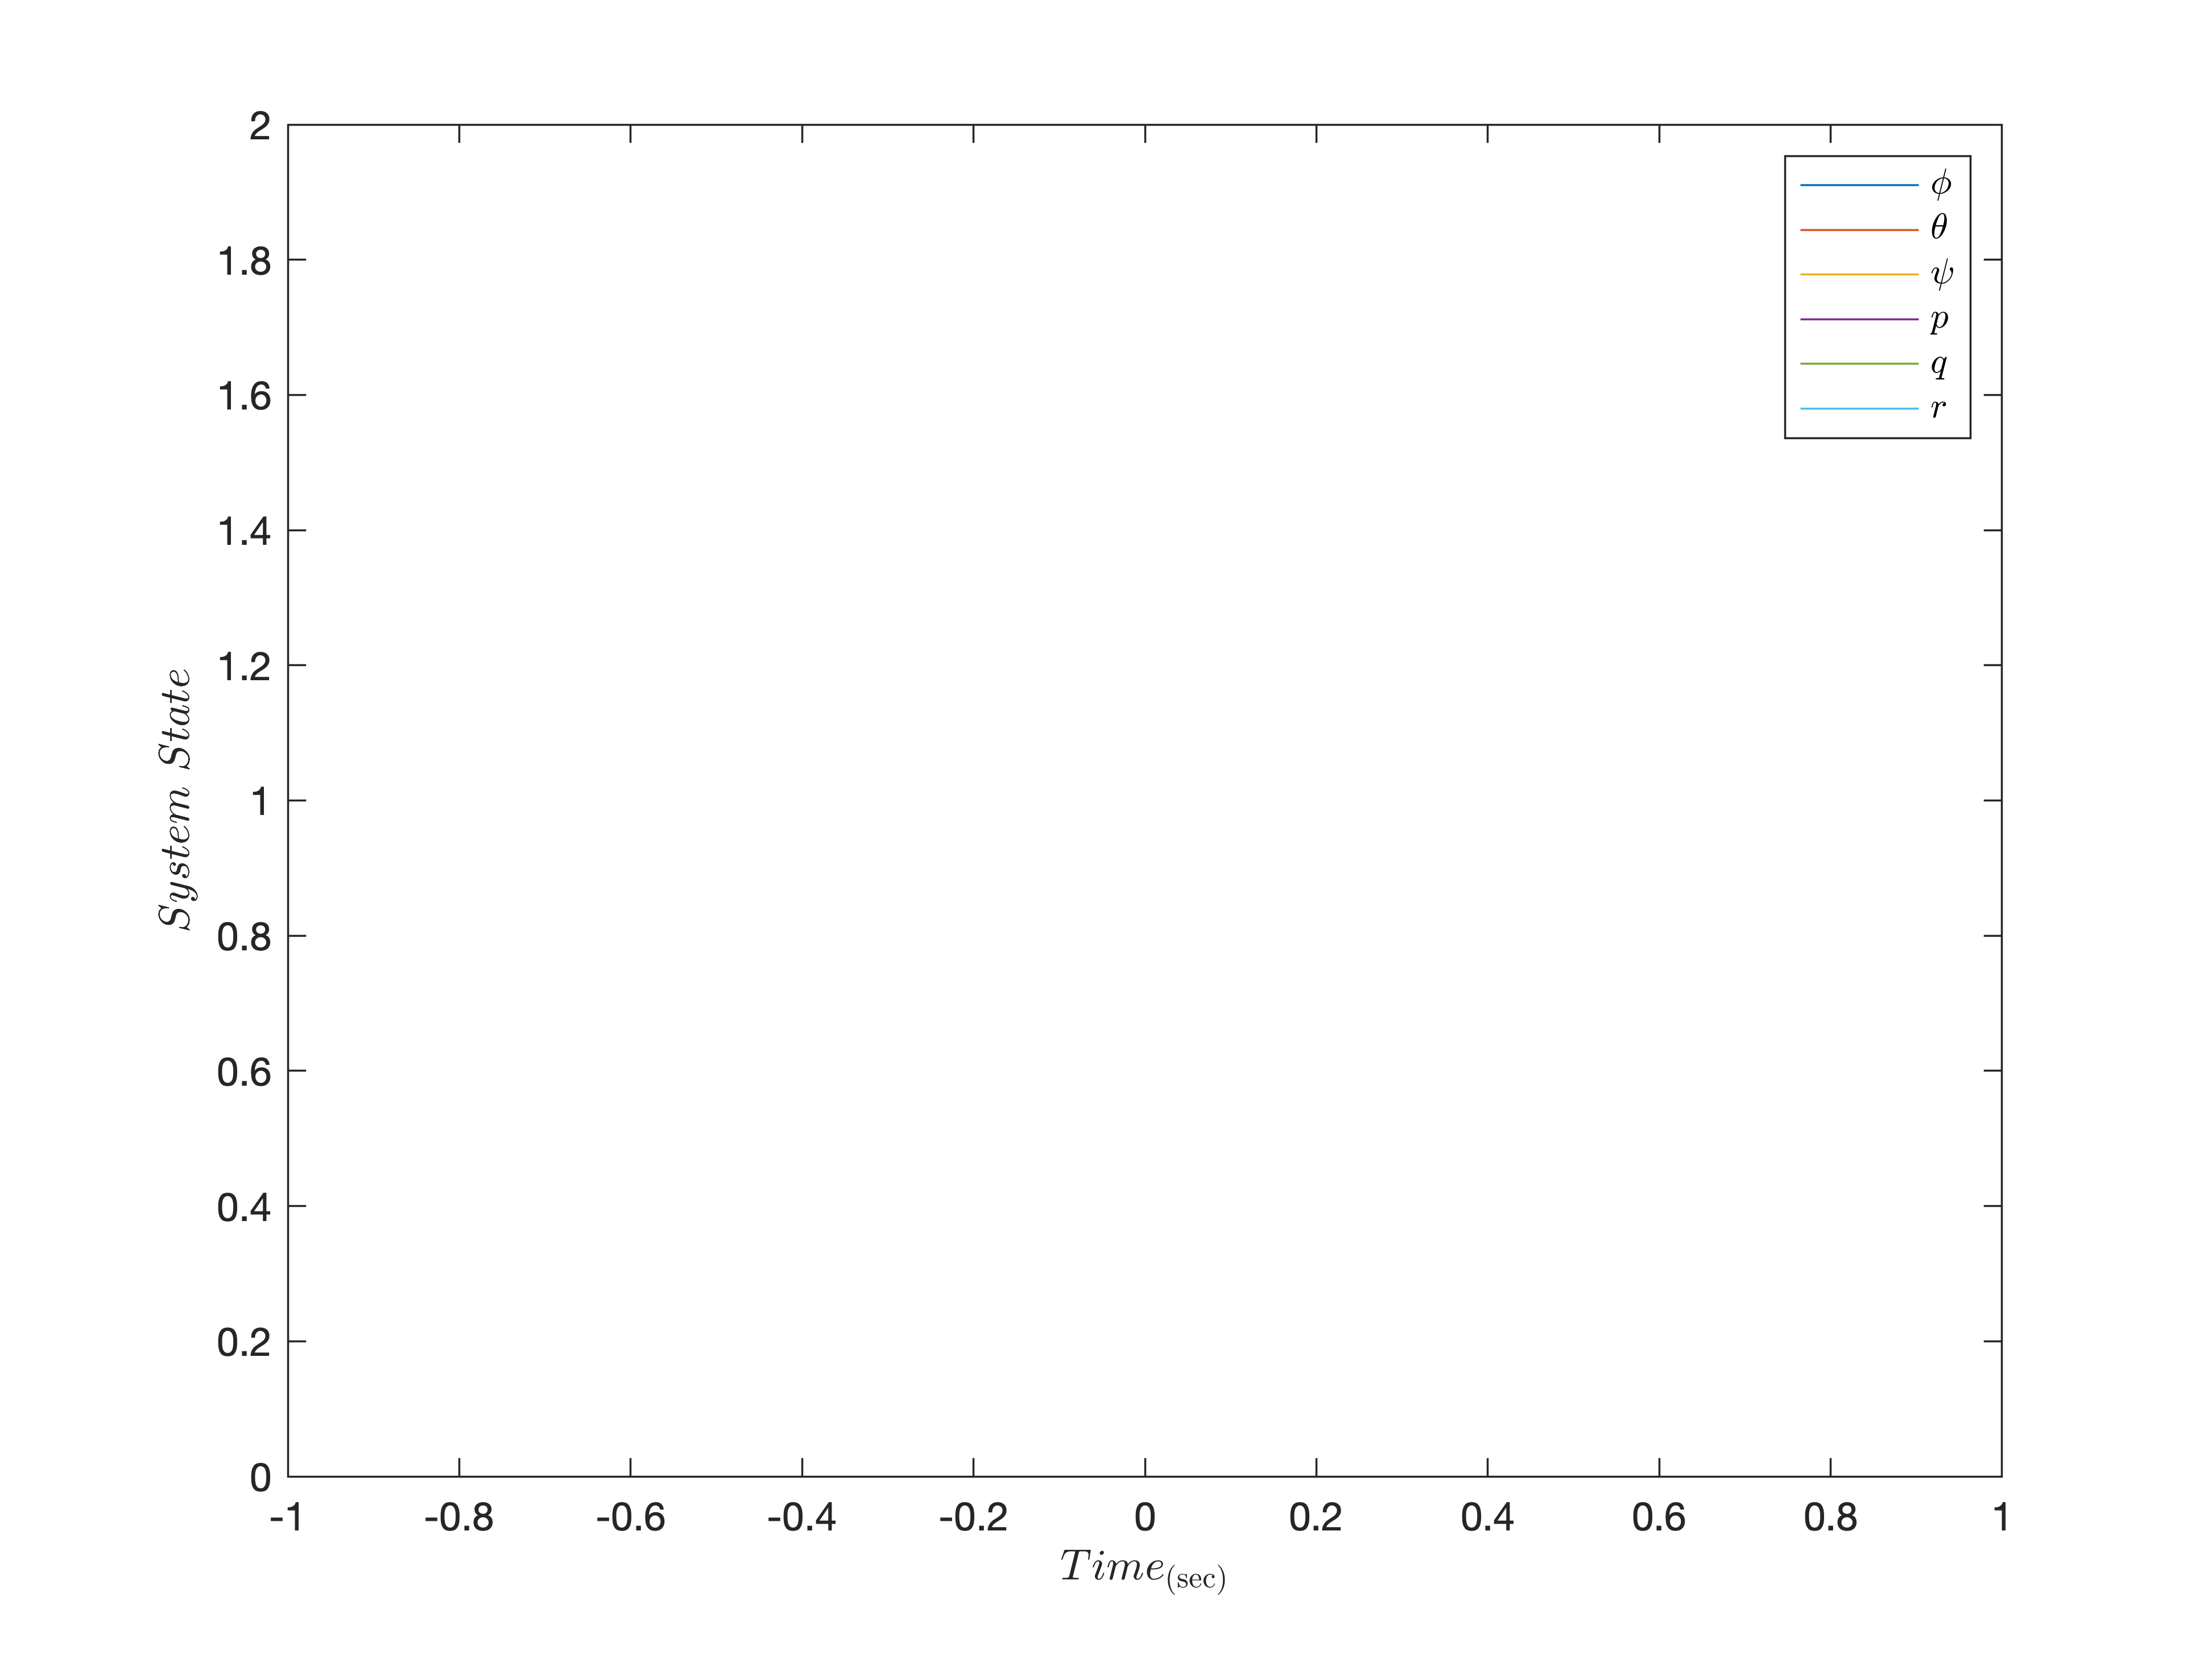
\includegraphics[width=12cm]{../Figure/LQDG/FeedBackLQDGall.png}
	\centering
	\caption{شبیه‌‌سازی چهارپره همراه با بازخورد در حالت انحراف تمامی وضعیت به اندازه یک رادیان(رادیان بر ثانیه)}
\end{figure}
\begin{figure}[H]
	\includegraphics[width=12cm]{../Figure/LQR/LQRall.png}
	\centering
	\caption{شبیه‌‌سازی چهارپره در کنترلر رگولاتور خطی در حالت انحراف تمامی وضعیت به اندازه یک رادیان(رادیان بر ثانیه)}
\end{figure}